%
% Exemplo LaTeX de artigo UNISINOS
%
% Elaborado com base nas orientações dadas no documento
% ``GUIA PARA ELABORAÇÃO DE TRABALHOS ACADÊMICOS''
% disponível no site da biblioteca da Unisinos.
% http://www.unisinos.br/biblioteca
%
% Os elementos textuais abaixo são apresentados na ordem em que devem
% aparecer no documento.  Repare que nem todos são obrigatórios - isso
% é devidamente indicado em cada caso.
%
% Comentários abaixo colocados entre aspas (`` '') foram
% extraídos diretamente do documento da biblioteca.
%
% Este documento é de domínio público.
%

%=======================================================================
% Declarações iniciais identificando a classe de documento e
% selecionando alguns pacotes adicionais.
%
% As opções disponíveis (separe-as com vírgulas, sem espaço) são:
% - twoside: Formata o documento para impressão frente-e-verso
%   (o default é somente-frente)
% - english,brazilian,french,german,etc.: idiomas usados no documento.
%   Deve ser colocado por último o idioma principal.
%=======================================================================
\documentclass[twoside,english,brazilian]{UNISINOSartigo}
\usepackage[utf8]{inputenc} % charset do texto (utf8, latin1, etc.)
\usepackage[T1]{fontenc} % encoding da fonte (afeta a sep. de sílabas)
\usepackage{graphicx} % comandos para gráficos e inclusão de figuras
\usepackage{bibentry} % para inserir refs. bib. no meio do texto

%=======================================================================

\unisinosbst
\usepackage{xcolor}
%\usepackage[alf]{abntcite}

%=======================================================================
% Início do documento.
%=======================================================================
\begin{document}
% Diferentemente do normal, os comandos a seguir devem vir aqui mesmo,
% e não antes do \begin{document} onde seria o lugar deles. 
\titulo{Quem são os profissionais "DevOps"  e quais são as suas competências ?}
\autor{Kim Bemfica Agliardi\footnote{Aluno do curso de Ciência da Computação.  Email: kim.agliardi@gmail.com}}
\autor{Christopher da Rosa Pohlmann \footnote{Orientador, professor da Unisinos, Mestre em Engenharia de Produção e Sistemas pela Universidade do Vale do Rio dos Sinos(2009)  Email: chrisp@unisinos.br}}

%=======================================================================
% Resumo em Português.
%
% A recomendação é para 150 a 250 palavras.
%=======================================================================
\begin{abstract}
Ao longo dos últimos anos a cultura de DevOps tem ganhado força no mercado de TI. O seu principal objetivo é o alinhamento entre as equipes de desenvolvimento e operação, para que juntos os times realizem entregas mais rápidas e de qualidade, por meio de ferramentas e responsabilidades previamente definidas. Trata-se de uma cultura de colaboração entre às equipes. Este estudo tem como objetivo realizar um panorama sobre os profissionais que estão trabalhando em organizações que praticam a cultura DevOps, entendendo qual é o seu nível de experiência no mercado de TI, entender quais práticas de DevOps estão em uso por estes profissionais, bem como mapear níveis de dificuldade encontrados por estes ao longo de implantações de ferramentas de automação, também mapeamos recursos são utilizados na busca de novos conhecimentos por estes profissionais.

\palavraschave{DevOps\@. Infraestrutura como código\@. Metódos Ágeis \@. Entrega Contínua \@. Integração Contínua. \@ }
\end{abstract}

%=======================================================================
% Introdução
%=======================================================================
\section{Introdução}
Ao longo dos últimos anos, foi possível observar um crescimento na importância das áreas de TI, fato que até então, não era verdade.  \citetexto{Beal2009}  lembra que "por muito tempo  a TI foi considerada um "centro de custo" e que em princípio não gerava qualquer retorno para o negócio", dando ênfase os altos valores de investimento em equipamentos e o pouco uso que se fazia destes.  Atualmente, as organizações vêm enfrentando um ambiente extremamente competitivo, inseridas em uma sociedade profundamente afetada pelos novos paradigmas introduzidos pela chamada sociedade da informação \citep{AudyFreitag08}.
A nova realidade provoca a reorganização intensa da sociedade, gerando modificações nas organizações. Neste contexto, as áreas de sistema de informação tem se tornado cada vez mais críticas,   dado o constante clima de mudança.

Com toda essa competitividade existente no mercado, mudanças de software tornaram-se comuns para as empresas, que até então, não estavam habituadas a realizar mudanças tão constantes em suas aplicações. O aumento no ritmo de entrega de software evidenciou a disparidade existente entre as equipes de desenvolvimento e operações de TI existentes nas organizações. Enquanto equipes de desenvolvimento, de um modo geral, possuem metodologias, frameworks e ferramentas bem estruturadas, que automatizam etapas de desenvolvimento de software e tratam do ciclo de vida de uma aplicação, equipes de operações de TI ainda  não estão tão bem estruturadas, realizando diversas tarefas de maneira manual e com uma baixa padronização. 

Confome \citetexto{Debois2008} observou as equipes de infraestrutura também podem adotar algumas das práticas já existentes e utilizadas por equipes de desenvolvimento, e a partir dos questionamentos levantados pelo artigo "Agile and Operations Infrastructure: How Infra-gile Are You?", foi gerada a lista de discussao "Agile-Sysadmin", que pode ser considerada uma semente inicial da cultura DevOps, que prega justamente a adoção de práticas de engenharia de software já consideradas maduras. Também podemos pensar em DevOps como uma evolução natural dos métodos ágeis, que foi estendido e passou à atender também áreas de operação. É importante salientar que diferente do movimento ágil ou ITIL, DevOps não possui uma "metodologia" para implementação, ou até mesmo, um manifesto, o que acaba tornando seu processo de adoção um pouco mais complexo, dado este contexto, diversos estudos buscam uma definição sobre o que é DevOps, quais são seus processos e práticas e quais são as características que as companhias buscam nos profissionais que vão compor estas equipes.

Desta forma, este estudo tem como objetivo analisar quais são as características dos profissionais que estão inseridos em ambientes que promovem a cultura DevOps, entendendo quais são suas habilidades técnicas, grupos de ferramentas utilizadas, experiências e dificuldades encontradas por estes profissionais para sustentar as práticas de automação que são aplicadas neste novo paradigma de trabalho.

A referida análise desdobra-se no seguintes objetivos específicos: (i) Identificar experiências prévias destes profissionais no mercado de TI, (ii) Identificar quais práticas de DevOps estão em uso por parte dos profissionais, (iii) Analisar como os profissionais estão se preparando (estudos) para este novo paradigma, e como buscam informações sobre novas ferramentas / práticas, (v) Analisar quais são as dificuldades e ganhos encontrados por estes profissionais na adoção deste novo paradigma

O \textbf{segundo capítulo} apresenta o referencial teórico, conceituando em linhas gerais o que é DevOps, quais são as características que esta cultura apresenta e uma breve descrição sobre as ferramentas utilizadas pelos profissionais.O \textbf{terceiro capítulo} apresenta-se as etapas de pesquisa. No \textbf{quarto capítulo} detalham-se os resultados do survey e por fim, no \textbf{quinto capítulo} seguem as conclusões.
%=======================================================================
% Referencial Teórico
%=======================================================================
\section{REFERENCIAL TEÓRICO}
	Ao longo deste capítulo, apresentam-se os principais conceitos sobre DevOps, como seus princípios, métodos e modelos, bem como a história de como surgiu o movimento.

\subsection{A relação entre Desenvolvimento  e Infraestrutura/Operação}

Com a pressão constante para entrega de valor por meio de software aos clientes, não é incomum que áreas de desenvolvimento e operações entrem em conflito. Enquanto desenvolvedores buscam pôr em produção o mais brevemente possível novas funcionalidades/sistemas, equipes de operação preocupam-se com a estabilidade, o que significa não realizar alterações em sistemas de produção frequentemente.
Segundo \citetexto{HUTTERMANN12}, estes conflitos geram barreiras culturais e organizacionais, que ocasionam as seguintes situações:

\begin{itemize}
\item Como o foco das equipes é diferente, a tensão entre as equipes aumenta e cada uma defende seus interesses individuais, sem pensar no todo;
\item A lacuna destes processo resulta em diferentes abordagens entre Dev/Ops sobre como gerenciar mudanças, colocá-las em produção e mantê-las funcionando;
\item  A origem dessa lacuna começa pelas próprias ferramentas utilizadas pelas equipes, que geralmente são diferentes.
\end{itemize}

Existe um termo na indústria que descreve esse tipo de comportamento como "O muro da confusão", que é causado justamente pela combinação de diferentes motivações (cada equipe defende o seu ponto), processos mal formulados e diferentes ferramentas de trabalho. Como cada equipe acredita estar fazendo o correto pelo negócio, as decisões ocorrem de maneira isolada e este "jogo de responsabilidades" ocorre.
% * <kim.agliardi@gmail.com> 2017-11-07T13:33:24.905Z:
% 
% Incluir citação Velocity09
% 
% ^ <kim.agliardi@gmail.com> 2017-11-07T13:33:37.858Z.

\begin{figure}[h]
    \centering
    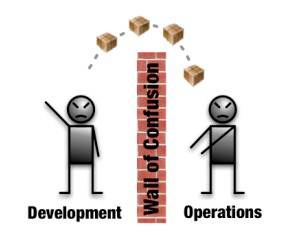
\includegraphics[scale=.9]{imagens/wallOfConfusion.jpg}
    \caption{Muro da confusão}
    \label{fig:Muro da confusão}
\end{figure}
É interessante observar que ao longo do tempo o processo de desenvolvimento de software sofreu diversos aprimoramentos, passando por modelos como o cascata (waterfall) até chegar no padrão que é visto hoje, que é baseado em metodologias ágeis. Já áreas de operações geralmente baseiam-se em métodos como ITIL (Information Technology Infrastructure Library), que possui processos processos claros e bem definidos para cada etapa de vida de um serviço. Essa diferença processual segue o mesmo descompasso que é visto no ferramental utilizado pelas equipes, enquanto métodos ágeis visam a entrega de pequenas partes de um sistema de maneira constante, gerando um grande número de alterações em um breve período de tempo por meio de suas "sprints", já ITIL, com o processo de gerênciamento de mudanças, prevê um modelo formal com reuniões e discussões entre às equipes antes da realização de alguma alteração. 
% * <kim.agliardi@gmail.com> 2017-11-11T15:25:58.747Z:
% 
% Ajustar essa seção com algumas referências e explicar a diferença de amadurencimento entre às áreas.
% 
% ^ <kim.agliardi@gmail.com> 2017-11-11T15:26:32.007Z.

\subsection{Métodos ágeis}
O movimento ágil começou com a escrita do \textbf{Manifesto Ágil} em 2001, e o nome "Agile" foi o nome dado ao conjunto de métodos de desenvolvimento de software que haviam sido desenhados para serem mais leves e flexíveis do que modelos como o cascata.
O que diz o  \textbf{Manifesto Ágil} :  \newline
Estamos descobrindo maneiras melhores de desenvolver 
software, fazendo-o nós mesmos e ajudando outros a 
fazerem o mesmo. Através deste trabalho, passamos a valorizar: 
\begin{itemize}
\item \textbf{Indivíduos e interações} mais que processos e ferramentas;
\item \textbf{Software em funcionamento} mais que documentação abrangente;
\item \textbf{Colaboração com o cliente} mais que negociação de contratos;
\item \textbf{Responder a mudanças} mais que seguir um plano
\end{itemize}
Ou seja, mesmo havendo valor nos itens à direita, valorizamos mais os itens à esquerda. \newline

É importante perceber que o principal objetivo do movimento ágil é enfatizar a colaboração, flexibilidade e como resultado final, diminuir o tempo de entrega de software, diminuir o valor gasto e fornecer um software de qualidade. Porém, os métodos ágeis não definem práticas para a disponibilização do software, o que acaba gerando uma lacuna entre as equipes de desenvolvimento e operação. Apesar do aumento de performance gerado pela adoção de práticas ágeis, existe a demora da fase de implantação do software, que em muitos casos, é causado pelo medo de "quebra" da aplicação à cada nova funcionalidade ou correção integrada a solução, por parte da equipe de operações, que tem como foco a estabilidade da aplicação.
O modelo ágil é próximo ao DevOps tanto no sentido cultural, isto é, o foco está nos indivíduos e na colaboração, quanto na redução de tempo de disponibilização de software. As práticas de integração contínua, entrega contínua, testes continuos e  infraestrutura como código, seguem justamente a ideia de não aguardar um ciclo inteiro para integrar, testar e disponibilizar, mas sim, integrar as funcionalidades assim que possível.

\subsection{ITIL}
A Information Technology Infrastructure Library (ITIL), é um conjunto de práticas definidas para o gerenciamento de serviços de TI . É uma publicação que contém 5 volumes que descrevem: Processos, procedimentos, tarefas e checklists e é utilizada por organizações para demonstrar conformidade e  medidas para melhoria de serviços. (citação Effective DevOps)
Sua primeira versão foi publicada no final dos anos 80, e o número de livros e práticas cresceu com o passar dos anos, sua última publicação (ITIL V3) foi realizada no ano de 2011, e esta versão contém livros sobre: Estratégias de serviço, Design de serviço, Transição de serviço, Operação de serviço e Melhoria continuada. 




\subsection{DevOps}
Nesta subseção aborda-se a origem do termo DevOps e suas principais características.

\subsubsection{A origem da cultura "DevOps"}
As "sementes" da cultura DevOps foram plantadas no ano de \textbf{2008}, pelo artigo publicado pelo belga  Patrick Debois, denominado "Agile and Operations Infrastructure: How Infra-gile Are You?" \citep{Debois2008}. A sua motivação para realização de sua pesquisa foi uma série de frustrações que ocorreram por conta de conflitos entre desenvolvedores e administradores de sistemas, ao longo de uma migração de um datacenter do governo belga.  No ano de 2008 na conferência sobre práticas ágeis (ajustar citação) Patrick Debois e Andrew Shafer apresentaram o trabalho construído e também criaram uma lista denominada \textbf{agile-sysadmin}, que inicialmente foi disseminada na Europa para discutir a adoção de metodologias ágeis na infrastrutura e entendermo como equipes de operação poderiam trabalhar no modelo ágil, acompanhando a equipe de desenvolvimento. Isto desencadeou uma série de estudos, confeencias e iniciativas sobre o assunto, que engajou a comunidade à torná-lo popular. 
Um outro marco importante para o DevOps foi a conferência Velocity da O'Really, realizada em 2009, aonde foi apresentado o trabalho \textbf{10+ Deploys per day: Dev and Ops Cooperation at Flickr}, por John Allspaw e Paul Hammond (inserir citação). Este trabalho foi um estudo de caso sobre a capacidade de implatanção de mudanças no Flickr após pôr em prática a colabração entre as equipes, priorizando a entrega de software de qualidade de maneira rápida e eficiente.
Esse estudo foi um marco para alavancar o movimento e nesta mesma conferência, surgiu a ideia de realizar o evento \textbf{DevOpsDays}, que é realizados em diversos países com grupos locais que tem como objetivo disseminar a cultura DevOps.

\subsubsection{O que é DevOps ?}

\textbf{DevOps} é um termo que se tornou uma "buzzword" no mercado e  por não ser prescritivo, muitas empresas tem apresentado a definição que lhes parece correta, bem como alguns profissionais que se entitulam "DevOps". 
Diferente das metodologias ágeis que possuem um manifesto ou ITIL que possui uma descrição sobre seus processos, não existe uma descrição exata sobre como "ser DevOps", pois ela é uma cultura definida por ideias e não por uma definição rigorosa e segundo \citetexto{Fallis2013} está em constante evolução, processos e ideias tem sido discutidos ao longo dos últimos anos e pelo que se observa na comunidade, a tendência é de que permaneça assim ao longo dos próximos anos.  \newline 
A definição proposta por \citep{Jabbari2016} é de que: DevOps é uma metodologia de desenvolvimento que busca eliminar os gap's existentes entre Desenvolvimento e Operações. Também pode ser dito como um paradigma, método ou conjunto de princípios e práticas que possibilitam uma melhor comunicação e colaboração, resultando em um trabalho em equipe eficiente entre as equipes de desenvolvedores e operadores.

Um acrônimo que é frequentemente citado nos grupos sobre DevOps é o CAMS, que significa \textbf{C}ulture, \textbf{A}utomation, \textbf{M}easurement and \textbf{S}haring. Ele é um framework muito útil e é frequentemente mencionado para demonstrar que DevOps não é apenas uma coisa única (como implementar uma ferramenta), mas uma abordagem mais ampla para prestação de serviço, Também trata como mehorar a colaboração, comunicação  e coordenação entre diferentes funções na organização. Segundo\cite{Willis}, temos as seguintes ideias sobre cada ponto:
\begin{itemize}
\item \textbf{Culture (Cultura)}: Pessoas e processos primeiro. Se você não tem cultura, todas as tentativas de automação serão inúteis, a mudança no mindset é fundamental para que a cultura prospere. Conforme a experiência de \textbf{(Ajustar citação ELBADY)} DevOps não funciona tão bem em estruturas de gerenciamento top-down. Como se trata de uma cultura inclusiva, é fundamental que exista uma aceitação/abertura  para diferentes ideias de diferentes níveis da organização. Uma comunicação abeta é frequentemente discutida como um ponto chave para impulsionar a cultura Devops. Walls (2013) diz: " A cultura DevOps foi criada por muita discussão e debate. Tradicionalmente, equipes técnicas interagem através de sistemas de chamados complexos e com procedimentos que podem ser considerados quase que rituais, o que às vezes requer intervenção da própria diretoria" (p.5);
\item \textbf{Automation (Automação)}: Este é um dos pontos de partida e mais discutidos para você entender cultura. Neste ponto, as ferramentas começão a formar uma "malha" de automação para DevOps. Ferramentas de gerenciamento de releases, provisionamento, gerênciamento de configuração, integração de sistemas, monitoramento e controle, e ferraamentas de orquestração são importantes pedaços desta malha;
\item \textbf{Measureament (Medidas)}: Se você não pode medir, você não pode melhorar. Uma implantação bem sucedida de DevOps mede tudo, o mais frequentemente possível. O core do monitoramento, é ser transparente sobre indicadores de performance que fazem a diferença. 
\item \textbf{Sharing (Compartilhar)}: Compartilhar é o "loopback" do ciclo CAMS. Criar uma cultura onde pessoas compartilham ideias e problema é o ponto crítico. Um outro ponto interessante é a maneira como histórias de sucesso estão sendo compartilhadas para ajudar a comunidade. É um ponto interessante pois além de atrair novos talentos, existe a crença de que, expondo ideias, você pode criar um excelente feedback aberto que, no final, ajuda a melhorar.
\end{itemize}
 
É possível observar que DevOps compartilha diversas características com o movimento ágil, especialmente sobre o foco em pessoas, interações e colaboração. Segundo \citep{Fallis2013}, embora DevOps tenha crescido em torno dos princípios do movimento ágil, ele é um movimento cultural separado, mergulhado na história da engenharia de software com um alcance mais amplo, do que a inclusão apenas de desenvolvedores. DevOps estende ideias ágeis e as aplica a uma organização inteira, não só ao processo de desenvolvimento.  
\subsection{Quais são as práticas que DevOps suporta? }

\textcolor{red}{Escrever um paragrafo apresentando as práticas DevOps. O que são estas práticas}

\textcolor{red}{Pode ser interessante colocar aquele desenho que o Matheus usou no artigo.}

O DevOps apresenta o conceito de práticas como ..... . Entre estas prática destacam-se a integração contínua, entrega contínua, etc.

\subsubsection{Integração contínua}
Integração contínua é um termo oriundo da metodologia ágil XP (eXtreme Programming) e utilizado em diversas metodologias. Consiste em: Integrar código alterado e/ou desenvolvido ao projeto principal na mesma frequência com que as funcionalidades são desenvolvidas, podendo ser realizado diversas vezes ao dia, ao invés de apenas uma vez. A ideia principal por trás deste processo é verificar se as alterações ou novas funcionalidades não criaram novos defeitos no projeto já existente e cada integração é verificada por um build automatizado (incluindo testes) para detectar erros de integração o mais rápido possível, muitos times acreditam que esse tipo de abordagem leva a uma significante redução nos problemas de integração e permite que um time desenvolva software coeso mais rapidamente \textbf{Citar Martin Fowler} . As informações sobre builds, testes e implantação são armazenadas em um pipeline de implantação. Neste pipeline de implantação, constam todos os dados referentes às fases do andamento da implantação. Para utilizar integração contínua, é obrigatório adotar algumas práticas, tais como: utilizar controle de versão, usar builds automatizados, usar estes isolados, realizar commits diários no repositório, utilizar um servidor de integração, executar testes automatizados e testes de infraestrutura. É interessante observar que diferente da integração "comum", aonde o software é considerado como não funcional até que a fase de testes valide que o mesmo funcione, já na integração contínua, o software é considerado funcionado, e a cada mudança no software, um conjunto de testes automatizados é executado para garantir seu funcionamento, permitindo assim, em caso de problemas, observar as falhas existentes de maneira mais ágil, diminuindo os prejuízos de correção.  
O objetivo desta prática é resolver problemas usuais de desenvolvimetno de software de maneirra mais rápida, pois integrando de maneira contínua, o processo se torna mais fluído, o que facilita na rastreabilidade de um problema. Organizações que não possuem este tipo de prática, tendem a realizar integrações após longos períodos de tempo, fazendo com que a rastreablidade de problemas e o tempo de resolução cresça considerávelmente. Em grande parte dos casos, o servidor de integração contínua também é responsável por aplicar testes automatizados e validar os check ins entregues por desenvolvedores, tanbpen realiza os testes de integração, desempenho e carga, caso o resultado destes seja positivo, a nova versão do software pode ser disponibilizada para o ambiente de produção.


\subsubsection{Entrega contínua}
Entrega contínua é a prática que garante a entrega de software por parte da equipe de desenvolvimento para o ambiente produtivo de forma confiável, previsível, visível e de modo mais automatizado possível, com riscos quantificados e compreendidos \cite{Humble2012}.  Ao invés de planejar grandes realeases e tudo que envolve este tipo de evento, times que praticam entrega contínua fornecem pequenas fatias de software para a produção com uma frequência maior do que entregas no modelo "formal, possívelmente várias vezes ao dia. Com esta prática, é possível entregar novas versões de software para produção de maneira mais fluída e em menor tempo, diminuindo o gap eixstente entre a etapa de desenvolvimento e disponibilização ao usuário final. Técnicas e práticas de entrega contínua reduzem tempo e riscos associados à entrega de novas versões de software para o usuário final, permitindo assim o aumento de feedback e a colaboração entre desenvolvedores, testadores e equipes de operação responsáveis pela entrega \cite{Humble2012}. \newline


A repetitividade e confiabilidade são fundamentais para a entrega contínua de software. Eles são obtidos através da automatização de todo processo , desde compilar e utilizar controle de versão para confiuração, até a implantação e testes da aplicação \citep{Humble2012}.
\subsubsection{Testes contínuos e automatizados}
Todos os processos em DevOps produzem código para a produção, assim que a etapa de desenvolvimento é finalizada. Isso requer que o código seja continuamente integrado e em paralelo, é necessário um conjunto de testes que trabalhe com a integração destas novas funcionalidades. Com implantações sendo realizadas de maneira mais rápida e frequente, é impossível executar testes manuais  de todas funcionalidades a cada release. Testar é uma atividade multifuncional que envolve todo o time e deve ser executada continuamente, desde o início do projeto \cite{Humble2012}.  (complementar....)
\subsubsection{Pipeline de implantação}
\subsubsection{Infraestrutura Como Código}
Infraestrutura como um código é uma abordagem para automação de infraestrutura baseada em práticas de desenvolvimento de software. A ênfase desta prática é em automação de rotinas consistentes e repetitivas, para provisionamento e mudança de configurações em sistemas. As mudanças são feitas em arquivos de definição e após isso, e estas são realizadas de maneira autônoma, incluindo a validação destas alterações.
A premissa das ferramentas modernas é a de que a infraestrutura pode ser tratada exatamente como um software.  Como resultado, todo o trabalho manual que era realizado, como por exemplo, a realização de alterações feitas diretamente em um servidor (ex: Configuração de uma variável de ambiente) deixa de ser realizado. Todas as alterações a serem realizadas devem estar em arquivos de configuração versionados em um repositório como Git ou similar, como qualquer outro código fonte \citep{Morris2016}. \newline
À partir destes arquivos de definição, um ambiente pode ser criado automaticamente do zero, com as mesmas características de outros ambientes da mesma versão. A qualquer momento, alguém pode olhar o histórico dos arquivos de definição e analisar as configurações do ambiente em uma determinada versão, o que de fato já pode ser considerado uma forma de "documentação viva" que corresponde ao exato estado do sistema naquele ponto.	\newline 
Baseado neste paradigma, criar e destruir ambientes frequentemente é uma boa prática. Um dos motivos é garantir que o ambiente sempre estará consistente com a configuração descrita. Além disso, reforça a cultura de que o ambiente de execução é descartável e não deve ser considerado uma "fonte de verdade" (source of truth).
Um benefícios de transformar a infraestrutura em código é a possibilidade de implementar a integração contínua de maneira adequada, permitindo a execução automática, isolada, e com testes de integração em ambientes com configurações idênticas à de produção. Também torna mais fácil o \textit{rollout} de uma aplicação do ambiente de homologação para o ambiente produtivo e como o processo é bem definido e bem descrito, podemos pensar na escalabilidade de uma aplicação em momentos de pico, de maneira automatizada. Em caso de problemas, o esforço é menor, pois para realizar o \textit{rollback} para a versão anterior da aplicação, seria necessário somente utilizar os arquivos de descrição. \newline
Como principal desvantagem, podemos pensar que para versionar a configuração, será exigido um tempo maior. A instalação manual de um servidor geralmente é rápida, porém, não é escalável. Já a definição da infra em arquivos de definição pode ser mais custosa, principalmente se o operador não for experiente no assunto.


%=======================================================================
% Conclusão
%=======================================================================
\section{Conclusão}
Não se esqueça de terminar o artigo com uma conclusão. :-)

%=======================================================================
% Resumo em língua estrangeira (sim, é aqui mesmo).
%
% O idioma usado aqui deve necessariamente aparecer nos parâmetros do
% \documentclass, no início do documento.
%=======================================================================


%=======================================================================
% Referências
%=======================================================================


\bibliography{TCC_DevOps}



\end{document}
